
\documentclass{article}
\usepackage[utf8]{inputenc}
\usepackage{graphicx}
\usepackage[T1]{fontenc}
\usepackage{lmodern}
\usepackage{listings}
\usepackage[numbers]{natbib} %IEEE
\usepackage{color}
\usepackage{hyperref}
\usepackage{soul}
\usepackage{float}
\usepackage{pgfplotstable}
\usepackage[font=itshape]{quoting}
\usepackage{booktabs}
\usepackage{amsmath}
\setcounter{MaxMatrixCols}{13}
\usepackage{multicol}
%\usepackage[table,xcdraw]{xcolor}

\usepackage{minted}
\usepackage[a4paper, total={6in, 8in}]{geometry}
\definecolor{dkgreen}{rgb}{0,0.6,0}
\definecolor{gray}{rgb}{0.5,0.5,0.5}
\definecolor{mauve}{rgb}{0.58,0,0.82}
\definecolor{backcolour}{rgb}{0.95,0.95,0.92}
\definecolor{codegreen}{rgb}{0,0.6,0}
% Define a custom style
\lstdefinestyle{myStyle}{
    backgroundcolor=\color{backcolour},   
    commentstyle=\color{codegreen},
    keywordstyle = \bfseries\color{mauve},
    basicstyle=\ttfamily\footnotesize,
    breakatwhitespace=false,         
    breaklines=true,                 
    keepspaces=true,                 
    numbers=left,       
    numbersep=5pt,                  
    showspaces=false,                
    showstringspaces=false,
    showtabs=false,                  
    tabsize=2,
}
\lstset{style=mystyle}

\title{Data Mining \& Machine Learning \\ \large Computer Exercise 11 - K-means}
\author{Steinarr Hrafn Höskuldsson}
\date{October 2022}
\newcommand{\mycomment}[1]{}

\begin{document}
\maketitle
\mycomment{
\begin{figure}[H]
    \centering
    \includegraphics[width=0.75\textwidth]{LAB3/Basic1.png}
    \caption{"Switch test" Breadboard set up}
    \label{fig:Switch_test}
\end{figure}

\lstinputlisting[caption=Defining 'ColorMatch' state, label={lst:colormatch}, language=Python, firstline=44, lastline=52]{LAB3/Basic.py}

}

\section*{Section 1.6}
\begin{figure}[h]
    \centering
    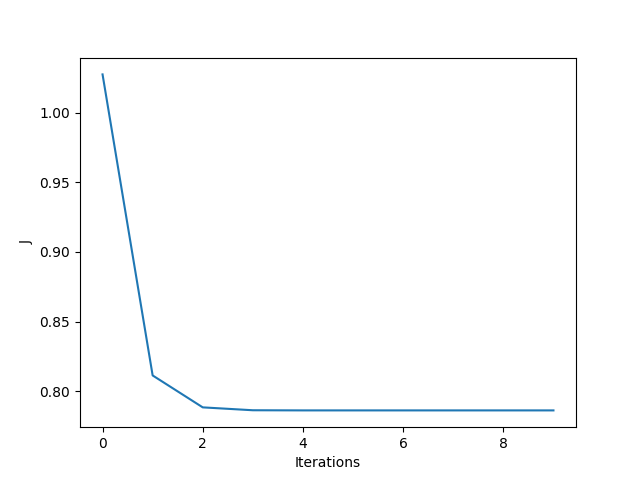
\includegraphics[width=0.75\textwidth]{11_k_means/1_6_1.png}
    \caption{J plotted by iterations}
    \label{fig:16}
\end{figure}

\section*{Section 1.7}
\begin{figure}[H]
    \centering
    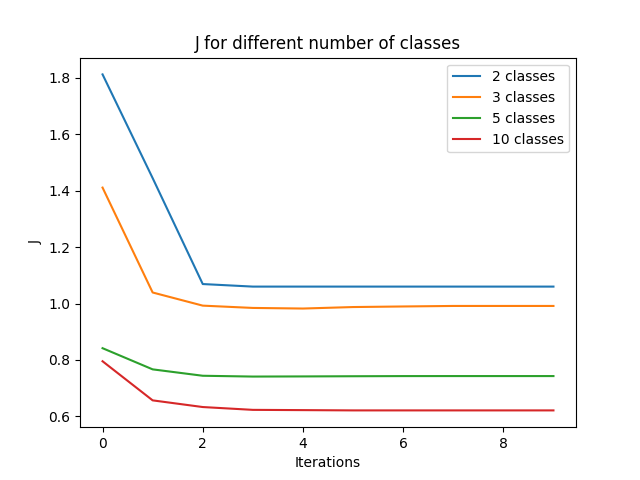
\includegraphics[width=0.75\textwidth]{11_k_means/1_7_1.png}
    \caption{J plotted by iterations for different number of classes}
    \label{fig:17}
\end{figure}

\section*{Section 1.8}
On Figure \ref{fig:17} we can see that using 10 classes better minimizes the objective function J.

The value of the objective funstion is calculated as the average distance from each datapoint to its classification prototype. And it gets smaller as we increase the classes. That is not because we are getting better results but rather simply because more prototypes occupy the same limited feature space thus decreasing the average distance.\\

If we were to set $k=n$, each prototype would be initialized as a unique data point and of course none of them would change since they are all closer to themselves rather then any other point. Choosing $k=n$ would however result in $J=0$ but is not a good strategy since it would result in each point classified in its own class which is, frankly, an utterly useless classification.

\section*{Section 1.10}
Training the K-means model with $k=3$ results in Accuracy$=82.67\%$ and Confusion matrix:
\\
CM = 
\begin{bmatrix}
         50 & 0 & 0\\
         0 & 42 & 8\\
         0 & 18 & 32
        \end{bmatrix}
\section*{Section 2.1}
\begin{figure}[H]
    \centering
    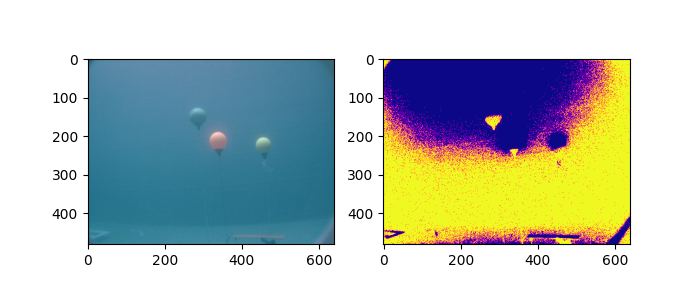
\includegraphics[width=0.75\textwidth]{11_k_means/2_1_1.png}
    \caption{K means applied to cluster an image based on color, using k=2}
    \label{fig:211}
\end{figure}
\begin{figure}[H]
    \centering
    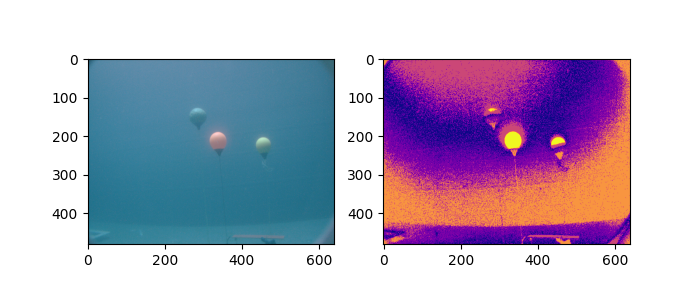
\includegraphics[width=0.75\textwidth]{11_k_means/2_1_2.png}
    \caption{K means applied to cluster an image based on color, using k=5}
    \label{fig:212}
\end{figure}
\begin{figure}[H]
    \centering
    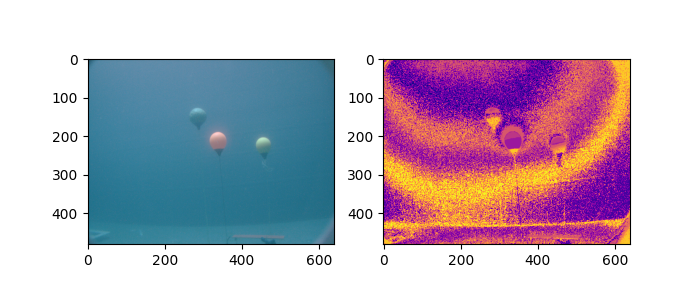
\includegraphics[width=0.75\textwidth]{11_k_means/2_1_3.png}
    \caption{K means applied to cluster an image based on color, using k=10}
    \label{fig:213}
\end{figure}
\begin{figure}[H]
    \centering
    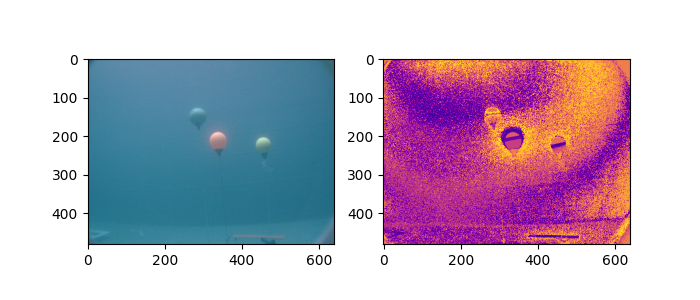
\includegraphics[width=0.75\textwidth]{11_k_means/2_1_4.png}
    \caption{K means applied to cluster an image based on color, using k=20}
    \label{fig:214}
\end{figure}

    
\end{document}

